\documentclass[UTF8,11pt]{ctexart}
\usepackage[a4paper,margin=22mm]{geometry}
\usepackage{amsmath,amssymb,bm,graphicx,adjustbox,fvextra,longtable,array}
\xeCJKDeclareCharClass{CJK}{"2160 -> "217F, "2460 -> "249B, "2200 -> "22FF}
\newcommand{\fitmath}[1]{\begin{adjustbox}{max width=\linewidth}$\displaystyle #1$\end{adjustbox}}
\setlength{\parindent}{0pt}\setlength{\parskip}{.65em}\renewcommand{\arraystretch}{1.3}
\sloppy\allowdisplaybreaks
\begin{document}
\section*{2016 年计算机统考 408 · 真题}
\subsection*{2016 年全国硕士研究生入学统一考试 计算机科学与技术学科联考计算机学科专业基础综合试题}

\subsection*{一、单项选择题（1～40 小题，每小题2 分，共80 分。下列每小题给出的四个选项中，只有一项符 合题目要求）}

1. 已知表头元素为 c 的单链表在内存中的存储状态如下表所示。


\begin{center}\begin{adjustbox}{max width=\linewidth}\begin{tabular}{|>{\raggedright\arraybackslash}p{\dimexpr(\linewidth-6\tabcolsep-4\arrayrulewidth)/3\relax}|>{\raggedright\arraybackslash}p{\dimexpr(\linewidth-6\tabcolsep-4\arrayrulewidth)/3\relax}|>{\raggedright\arraybackslash}p{\dimexpr(\linewidth-6\tabcolsep-4\arrayrulewidth)/3\relax}|}\hline
地址 & 元素 & 链接地址\\\hline
1000H & a & 1010H\\\hline
1004H & b & 100CH\\\hline
1008H & c & 1000H\\\hline
100CH & d & NULL\\\hline
1010H & e & 1004H\\\hline
1014H &  & \\\hline\end{tabular}\end{adjustbox}\end{center}

现将 f 存放于 1014H 处并插入到单链表中，若 f 在逻辑上位于 a 和 e 之间，则 a、e、f 的“链接地址”依次是\_\_\_\_\_\_。


\begin{center}\begin{tabular}{>{\raggedright\arraybackslash}p{\dimexpr(\linewidth-4\tabcolsep)/2\relax}>{\raggedright\arraybackslash}p{\dimexpr(\linewidth-4\tabcolsep)/2\relax}}
\textbf{A.} 1010H，1014H，1004H & \textbf{B.} 1010H，1004H，1014H\\[.35em]
\textbf{C.} 1014H，1010H，1004H & \textbf{D.} 1014H，1004H，1010H\\[.35em]\end{tabular}\end{center}

2. 已知一个带有表头结点的双向循环链表 L，结点结构为 prev、data、next，其中，prev 和 next 分别是指向其直接前驱和直接后继结点的指针。现要删除指针 p 所指的结点，正确的语句序列是\_\_\_\_\_\_。


\begin{center}\begin{tabular}{>{\raggedright\arraybackslash}p{\dimexpr(\linewidth-4\tabcolsep)/2\relax}>{\raggedright\arraybackslash}p{\dimexpr(\linewidth-4\tabcolsep)/2\relax}}
\textbf{A.} p->next->prev=p->prev; p->prev->next=p->prev; free(p); & \textbf{B.} p->next->prev=p->next; p->prev->next=p->next; free(p);\\[.35em]
\textbf{C.} p->next->prev=p->next; p->prev->next=p->prev; free(p); & \textbf{D.} p->next->prev=p->prev; p->prev->next=p->next; free(p);\\[.35em]\end{tabular}\end{center}

3. 设有下图所示的火车车轨，入口到出口之间有n 条轨道，列车的行进方向均为从左至右，列车可 驶入任意一条轨道。现有编号为1～9 的9 列列车，驶入的次序依次是8，4，2，5，3，9，1， 6，7。若期望驶出的次序依次为1～9，则n 至少是\_\_\_\_\_\_。


\begin{center}\begin{tabular}{>{\raggedright\arraybackslash}p{\dimexpr(\linewidth-8\tabcolsep)/4\relax}>{\raggedright\arraybackslash}p{\dimexpr(\linewidth-8\tabcolsep)/4\relax}>{\raggedright\arraybackslash}p{\dimexpr(\linewidth-8\tabcolsep)/4\relax}>{\raggedright\arraybackslash}p{\dimexpr(\linewidth-8\tabcolsep)/4\relax}}
\textbf{A.} 2 & \textbf{B.} 3 & \textbf{C.} 4 & \textbf{D.} 5\\[.35em]\end{tabular}\end{center}

\begin{center}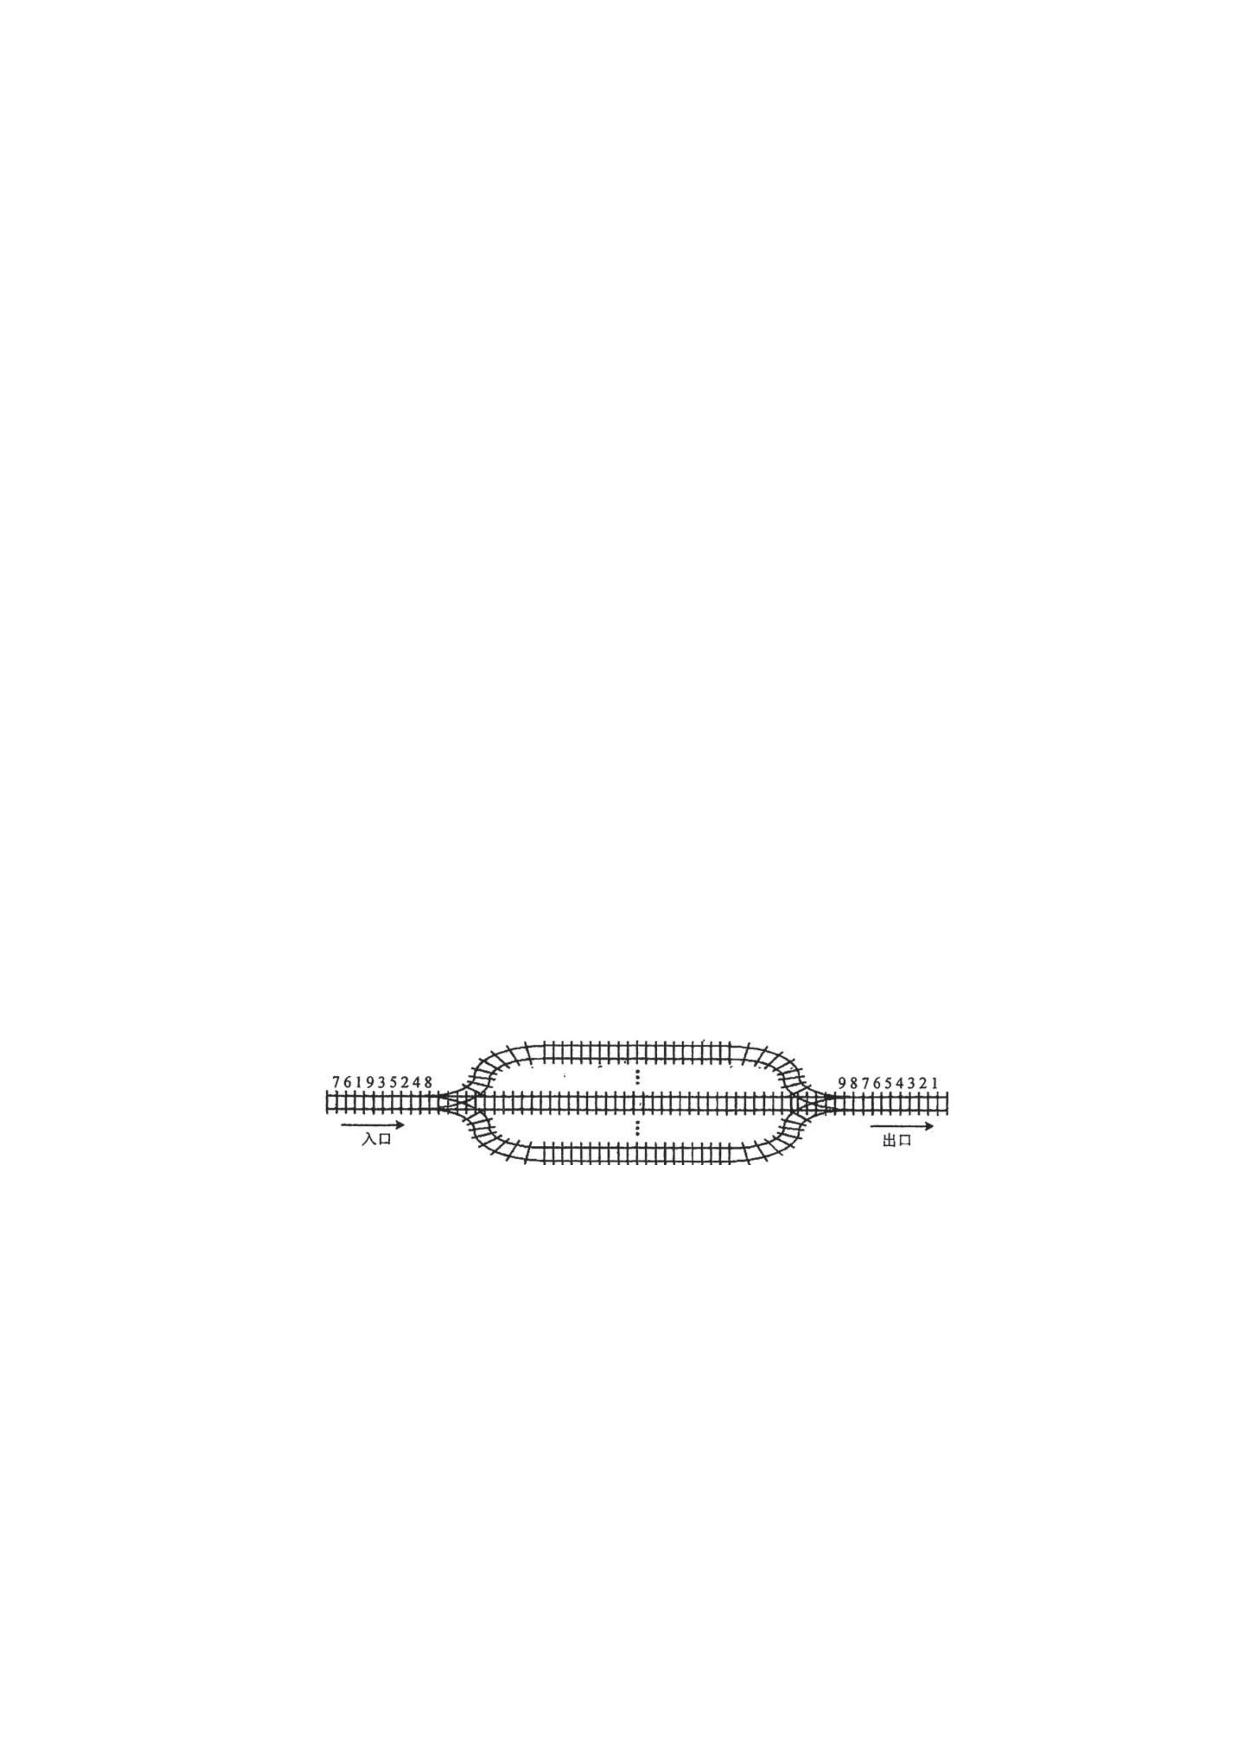
\includegraphics[width=.65\linewidth,height=.4\textheight,keepaspectratio]{../assets/figures/2016-questions-p001-b007.pdf}\end{center}

4. 有一个 100 阶的三对角矩阵 \(\displaystyle M\)，其元素 \(\displaystyle m_{i,\allowbreak j}\;(1\le i\le100,\allowbreak 1\le j\le100)\) 按行优先依次压缩存入下标从 0 开始的一维数组 \(\displaystyle N\) 中。元素 \(\displaystyle m_{30,\allowbreak 30}\) 在 \(\displaystyle N\) 中的下标是\_\_\_\_\_\_。


\begin{center}\begin{tabular}{>{\raggedright\arraybackslash}p{\dimexpr(\linewidth-8\tabcolsep)/4\relax}>{\raggedright\arraybackslash}p{\dimexpr(\linewidth-8\tabcolsep)/4\relax}>{\raggedright\arraybackslash}p{\dimexpr(\linewidth-8\tabcolsep)/4\relax}>{\raggedright\arraybackslash}p{\dimexpr(\linewidth-8\tabcolsep)/4\relax}}
\textbf{A.} 86 & \textbf{B.} 87 & \textbf{C.} 88 & \textbf{D.} 89\\[.35em]\end{tabular}\end{center}

5. 若森林F 有15 条边、25 个结点，则F 包含树的个数是\_\_\_\_\_\_。


\begin{center}\begin{tabular}{>{\raggedright\arraybackslash}p{\dimexpr(\linewidth-8\tabcolsep)/4\relax}>{\raggedright\arraybackslash}p{\dimexpr(\linewidth-8\tabcolsep)/4\relax}>{\raggedright\arraybackslash}p{\dimexpr(\linewidth-8\tabcolsep)/4\relax}>{\raggedright\arraybackslash}p{\dimexpr(\linewidth-8\tabcolsep)/4\relax}}
\textbf{A.} 8 & \textbf{B.} 9 & \textbf{C.} 10 & \textbf{D.} 11\\[.35em]\end{tabular}\end{center}

6. 下列选项中，不是下图深度优先搜索序列的是\_\_\_\_\_\_。


\begin{center}\begin{tabular}{>{\raggedright\arraybackslash}p{\dimexpr(\linewidth-4\tabcolsep)/2\relax}>{\raggedright\arraybackslash}p{\dimexpr(\linewidth-4\tabcolsep)/2\relax}}
\textbf{A.} V1, V5, V4, V3, V2 & \textbf{B.} V1, V3, V2, V5, V4\\[.35em]
\textbf{C.} V1, V2, V5, V4, V3 & \textbf{D.} V1, V2, V3,V4, V5\\[.35em]\end{tabular}\end{center}

\begin{center}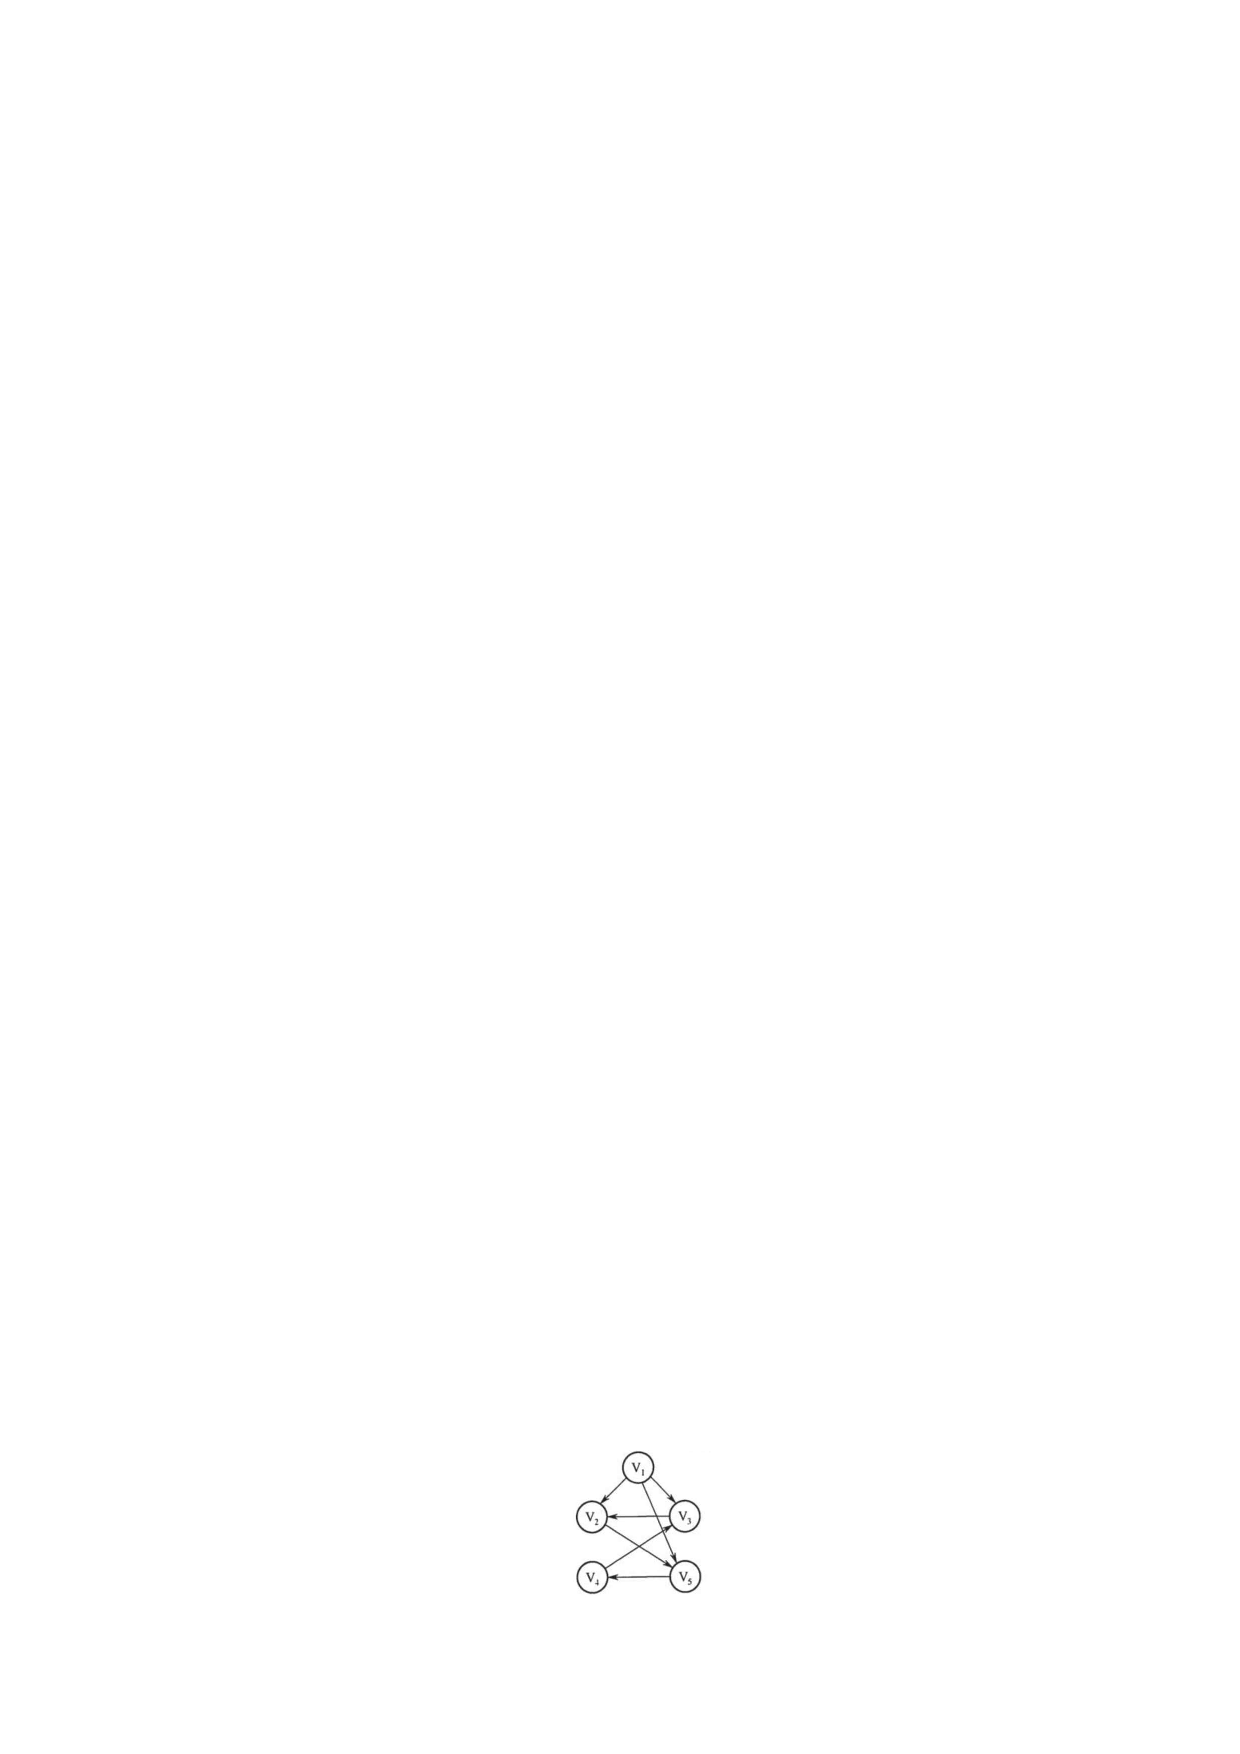
\includegraphics[width=.65\linewidth,height=.4\textheight,keepaspectratio]{../assets/figures/2016-questions-p001-b011.pdf}\end{center}

7. 若将 \(\displaystyle n\) 个顶点、\(\displaystyle e\) 条弧的有向图采用邻接表存储，则拓扑排序算法的时间复杂度是\_\_\_\_\_\_。


\begin{center}\begin{tabular}{>{\raggedright\arraybackslash}p{\dimexpr(\linewidth-8\tabcolsep)/4\relax}>{\raggedright\arraybackslash}p{\dimexpr(\linewidth-8\tabcolsep)/4\relax}>{\raggedright\arraybackslash}p{\dimexpr(\linewidth-8\tabcolsep)/4\relax}>{\raggedright\arraybackslash}p{\dimexpr(\linewidth-8\tabcolsep)/4\relax}}
\textbf{A.} \(\displaystyle O(n)\) & \textbf{B.} \(\displaystyle O(n+e)\) & \textbf{C.} \(\displaystyle O(n^2)\) & \textbf{D.} \(\displaystyle O(ne)\)\\[.35em]\end{tabular}\end{center}

8. 使用迪杰斯特拉(Dijkstra)算法求下图中从顶点1 到其他各顶点的最短路径，依次得到的各最短路 径的目标顶点是\_\_\_\_\_\_。


\begin{center}\begin{tabular}{>{\raggedright\arraybackslash}p{\dimexpr(\linewidth-8\tabcolsep)/4\relax}>{\raggedright\arraybackslash}p{\dimexpr(\linewidth-8\tabcolsep)/4\relax}>{\raggedright\arraybackslash}p{\dimexpr(\linewidth-8\tabcolsep)/4\relax}>{\raggedright\arraybackslash}p{\dimexpr(\linewidth-8\tabcolsep)/4\relax}}
\textbf{A.} 5, 2, 3, 4, 6 & \textbf{B.} 5, 2, 3, 6, 4 & \textbf{C.} 5, 2, 4, 3, 6 & \textbf{D.} 5, 2, 6, 3, 4\\[.35em]\end{tabular}\end{center}

\begin{center}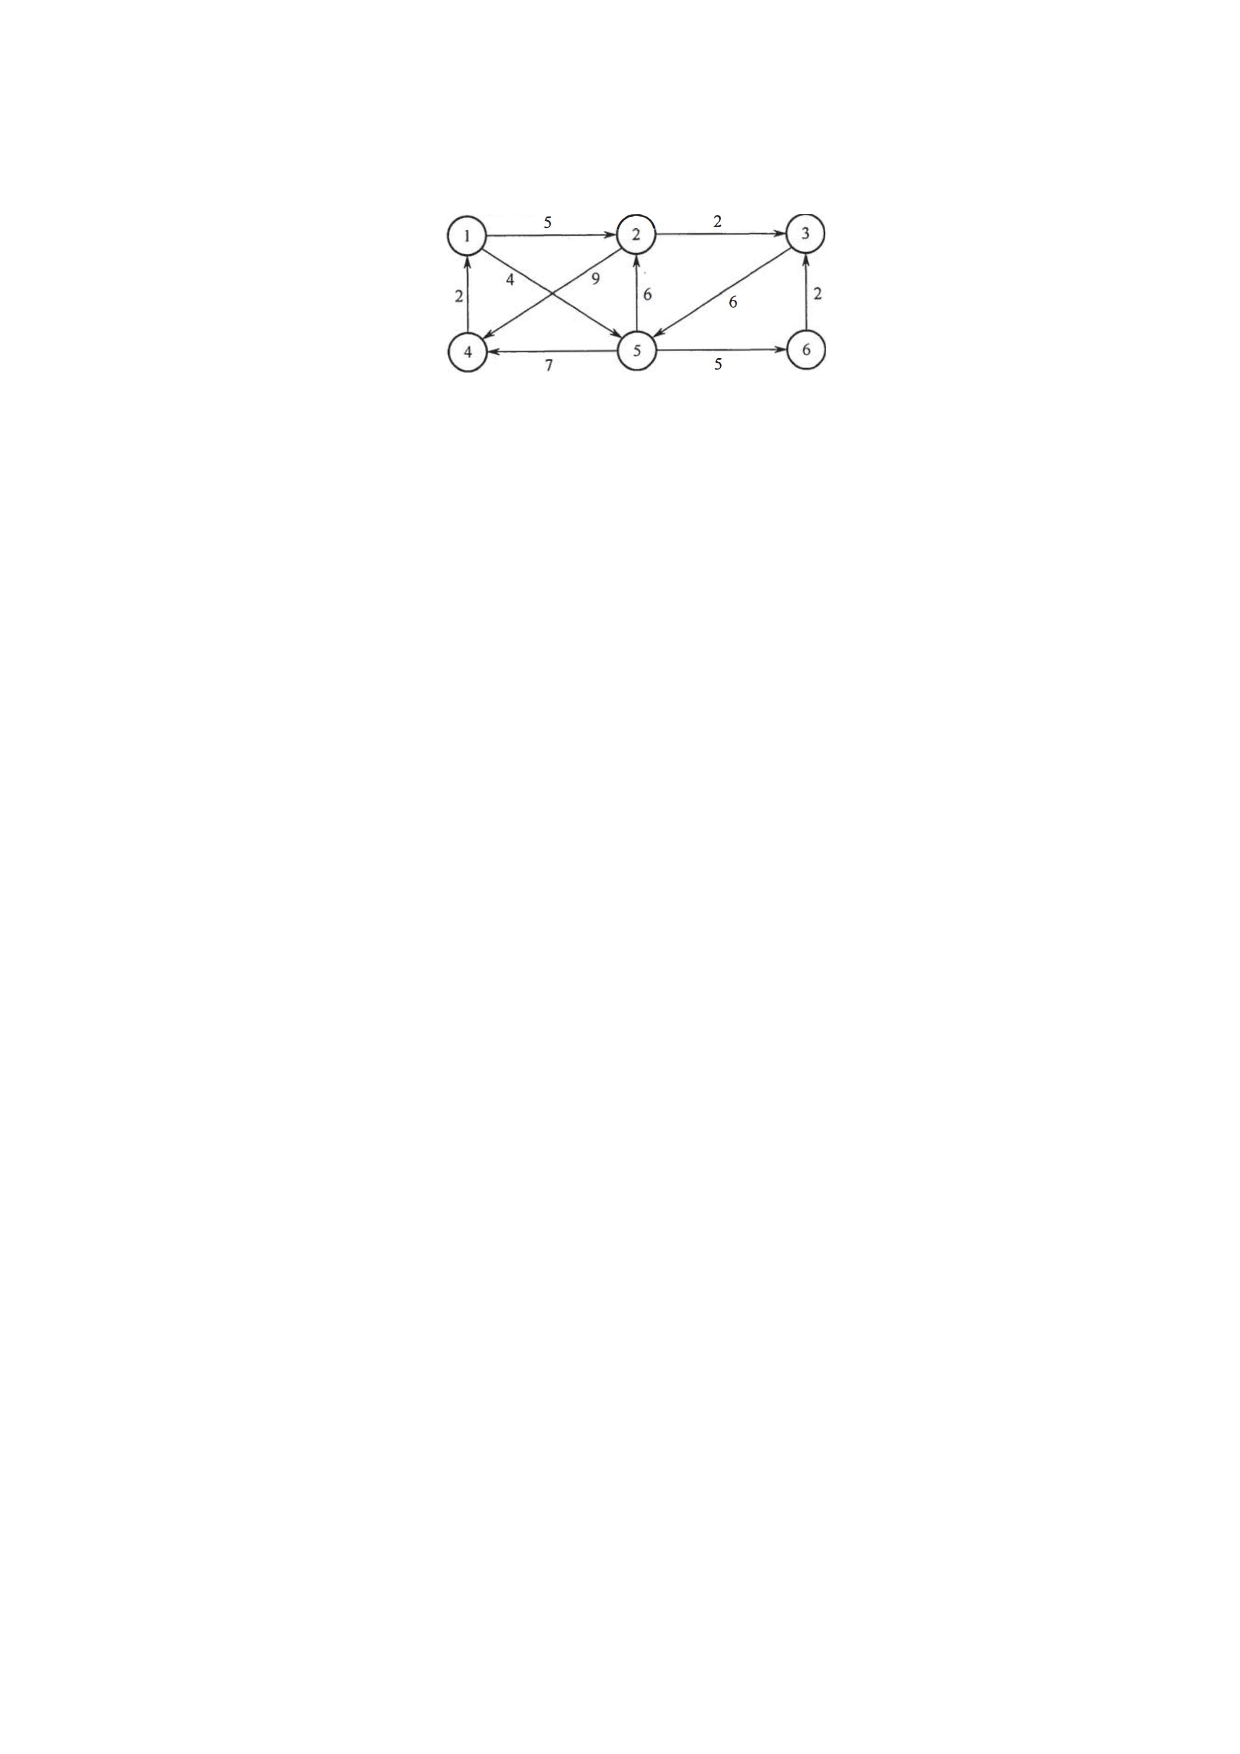
\includegraphics[width=.65\linewidth,height=.4\textheight,keepaspectratio]{../assets/figures/2016-questions-p002-b002.pdf}\end{center}

9. 在有 \(\displaystyle n\;(n>1000)\) 个元素的升序数组 A 中查找关键字 x。查找算法的伪代码如下所示。


\begin{Verbatim}[breaklines,breakanywhere,fontsize=\small]
k=0;
while (k<n 且 A[k]<x) k=k+3;
if (k<n 且 A[k]==x) 查找成功;
else if (k-1<n 且 A[k-1]==x) 查找成功;
else if (k-2<n 且 A[k-2]==x) 查找成功;
else 查找失败;
\end{Verbatim}

本算法与折半查找算法相比，有可能具有更少比较次数的情形是\_\_\_\_\_\_。


\begin{center}\begin{tabular}{>{\raggedright\arraybackslash}p{\dimexpr(\linewidth-4\tabcolsep)/2\relax}>{\raggedright\arraybackslash}p{\dimexpr(\linewidth-4\tabcolsep)/2\relax}}
\textbf{A.} 当 x 不在数组中 & \textbf{B.} 当 x 接近数组开头处\\[.35em]
\textbf{C.} 当 x 接近数组结尾处 & \textbf{D.} 当 x 位于数组中间位置\\[.35em]\end{tabular}\end{center}

10.B+树不同于B 树的特点之一是\_\_\_\_\_\_。


\begin{center}\begin{tabular}{>{\raggedright\arraybackslash}p{\dimexpr(\linewidth-4\tabcolsep)/2\relax}>{\raggedright\arraybackslash}p{\dimexpr(\linewidth-4\tabcolsep)/2\relax}}
\textbf{A.} 能支持顺序查找 & \textbf{B.} 结点中含有关键字\\[.35em]
\textbf{C.} 根结点至少有两个分支 & \textbf{D.} 所有叶结点都在同一层上\\[.35em]\end{tabular}\end{center}

11.对10TB 的数据文件进行排序，应使用的方法是\_\_\_\_\_\_。


\begin{center}\begin{tabular}{>{\raggedright\arraybackslash}p{\dimexpr(\linewidth-8\tabcolsep)/4\relax}>{\raggedright\arraybackslash}p{\dimexpr(\linewidth-8\tabcolsep)/4\relax}>{\raggedright\arraybackslash}p{\dimexpr(\linewidth-8\tabcolsep)/4\relax}>{\raggedright\arraybackslash}p{\dimexpr(\linewidth-8\tabcolsep)/4\relax}}
\textbf{A.} 希尔排序 & \textbf{B.} 堆排序 & \textbf{C.} 快速排序 & \textbf{D.} 归并排序\\[.35em]\end{tabular}\end{center}

12.将高级语言源程序转换为机器级目标代码文件的程序是\_\_\_\_\_\_。


\begin{center}\begin{tabular}{>{\raggedright\arraybackslash}p{\dimexpr(\linewidth-8\tabcolsep)/4\relax}>{\raggedright\arraybackslash}p{\dimexpr(\linewidth-8\tabcolsep)/4\relax}>{\raggedright\arraybackslash}p{\dimexpr(\linewidth-8\tabcolsep)/4\relax}>{\raggedright\arraybackslash}p{\dimexpr(\linewidth-8\tabcolsep)/4\relax}}
\textbf{A.} 汇编程序 & \textbf{B.} 链接程序 & \textbf{C.} 编译程序 & \textbf{D.} 解释程序\\[.35em]\end{tabular}\end{center}

13. 有如下 C 语言程序段：


\begin{Verbatim}[breaklines,breakanywhere,fontsize=\small]
short si = -32767;
unsigned short usi = si;
\end{Verbatim}

执行上述两条语句后，usi 的值为\_\_\_\_\_\_。


\begin{center}\begin{tabular}{>{\raggedright\arraybackslash}p{\dimexpr(\linewidth-8\tabcolsep)/4\relax}>{\raggedright\arraybackslash}p{\dimexpr(\linewidth-8\tabcolsep)/4\relax}>{\raggedright\arraybackslash}p{\dimexpr(\linewidth-8\tabcolsep)/4\relax}>{\raggedright\arraybackslash}p{\dimexpr(\linewidth-8\tabcolsep)/4\relax}}
\textbf{A.} −32767 & \textbf{B.} 32767 & \textbf{C.} 32768 & \textbf{D.} 32769\\[.35em]\end{tabular}\end{center}

14.计算机字长为32 位，按字节编址，采用小端（Little Endian）方式存放数据。假定有一个double 型变量，其机器数表示为1122 3344 5566 7788H，存放在0000 8040H 开始的连续存储单元中， 则存储单元0000 8046H 中存放的是\_\_\_\_\_\_。


\begin{center}\begin{tabular}{>{\raggedright\arraybackslash}p{\dimexpr(\linewidth-8\tabcolsep)/4\relax}>{\raggedright\arraybackslash}p{\dimexpr(\linewidth-8\tabcolsep)/4\relax}>{\raggedright\arraybackslash}p{\dimexpr(\linewidth-8\tabcolsep)/4\relax}>{\raggedright\arraybackslash}p{\dimexpr(\linewidth-8\tabcolsep)/4\relax}}
\textbf{A.} 22H & \textbf{B.} 33H & \textbf{C.} 77H & \textbf{D.} 66H\\[.35em]\end{tabular}\end{center}

15. 有如下 C 语言程序段：


\begin{Verbatim}[breaklines,breakanywhere,fontsize=\small]
for (k=0; k<1000; k++)
    a[k] = a[k]+32
\end{Verbatim}

若数组 a 及变量 k 均为 int 型，int 型数据占 4B，数据 Cache 采用直接映射方式，数据区大小为 1KB、块大小为 16B，该程序段执行前 Cache 为空，则该程序段执行过程中访问数组 a 的 Cache 缺失率约为\_\_\_\_\_\_。


\begin{center}\begin{tabular}{>{\raggedright\arraybackslash}p{\dimexpr(\linewidth-8\tabcolsep)/4\relax}>{\raggedright\arraybackslash}p{\dimexpr(\linewidth-8\tabcolsep)/4\relax}>{\raggedright\arraybackslash}p{\dimexpr(\linewidth-8\tabcolsep)/4\relax}>{\raggedright\arraybackslash}p{\dimexpr(\linewidth-8\tabcolsep)/4\relax}}
\textbf{A.} 1.\allowbreak{}25％ & \textbf{B.} 2.\allowbreak{}5％ & \textbf{C.} 12.\allowbreak{}5％ & \textbf{D.} 25％\\[.35em]\end{tabular}\end{center}

16.某存储器容量为64KB，按字节编址，地址4000H～5FFFH 为ROM 区，其余为RAM 区。若采 用8K×4 位的SRAM 芯片进行设计，则需要该芯片的数量是\_\_\_\_\_\_。


\begin{center}\begin{tabular}{>{\raggedright\arraybackslash}p{\dimexpr(\linewidth-8\tabcolsep)/4\relax}>{\raggedright\arraybackslash}p{\dimexpr(\linewidth-8\tabcolsep)/4\relax}>{\raggedright\arraybackslash}p{\dimexpr(\linewidth-8\tabcolsep)/4\relax}>{\raggedright\arraybackslash}p{\dimexpr(\linewidth-8\tabcolsep)/4\relax}}
\textbf{A.} 7 & \textbf{B.} 8 & \textbf{C.} 14 & \textbf{D.} 16\\[.35em]\end{tabular}\end{center}

17. 某指令格式如下所示。


\begin{center}\begin{adjustbox}{max width=\linewidth}\begin{tabular}{|>{\raggedright\arraybackslash}p{\dimexpr(\linewidth-8\tabcolsep-5\arrayrulewidth)/4\relax}|>{\raggedright\arraybackslash}p{\dimexpr(\linewidth-8\tabcolsep-5\arrayrulewidth)/4\relax}|>{\raggedright\arraybackslash}p{\dimexpr(\linewidth-8\tabcolsep-5\arrayrulewidth)/4\relax}|>{\raggedright\arraybackslash}p{\dimexpr(\linewidth-8\tabcolsep-5\arrayrulewidth)/4\relax}|}\hline
OP & M & I & D\\\hline\end{tabular}\end{adjustbox}\end{center}

其中 M 为寻址方式，I 为变址寄存器编号，D 为形式地址。若采用先变址后间址的寻址方式，则操作数的有效地址是\_\_\_\_\_\_。


\begin{center}\begin{tabular}{>{\raggedright\arraybackslash}p{\dimexpr(\linewidth-8\tabcolsep)/4\relax}>{\raggedright\arraybackslash}p{\dimexpr(\linewidth-8\tabcolsep)/4\relax}>{\raggedright\arraybackslash}p{\dimexpr(\linewidth-8\tabcolsep)/4\relax}>{\raggedright\arraybackslash}p{\dimexpr(\linewidth-8\tabcolsep)/4\relax}}
\textbf{A.} I+D & \textbf{B.} (I)+D & \textbf{C.} ((I)+D) & \textbf{D.} ((I))+D\\[.35em]\end{tabular}\end{center}

18.某计算机主存空间为4GB，字长为32 位，按字节编址，采用32 位字长指令字格式。若指令按 字边界对齐存放，则程序计数器（PC）和指令寄存器（IR）的位数至少分别是\_\_\_\_\_\_。


\begin{center}\begin{tabular}{>{\raggedright\arraybackslash}p{\dimexpr(\linewidth-8\tabcolsep)/4\relax}>{\raggedright\arraybackslash}p{\dimexpr(\linewidth-8\tabcolsep)/4\relax}>{\raggedright\arraybackslash}p{\dimexpr(\linewidth-8\tabcolsep)/4\relax}>{\raggedright\arraybackslash}p{\dimexpr(\linewidth-8\tabcolsep)/4\relax}}
\textbf{A.} 30、30 & \textbf{B.} 30、32 & \textbf{C.} 32、30 & \textbf{D.} 32、32\\[.35em]\end{tabular}\end{center}

19. 在无转发机制的五段基本流水线（取指、译码/读寄存器、运算、访/写回寄存器）中，下列指令序列存在数据冒险的指令对是\_\_\_\_\_\_。


\begin{Verbatim}[breaklines,breakanywhere,fontsize=\small]
I1: add R1, R2, R3;  (R2)+(R3)→R1
I2: add R5, R2, R4;  (R2)+(R4)→R5
I3: add R4, R5, R3;  (R5)+(R3)→R4
I4: add R5, R2, R6;  (R2)+(R6)→R5
\end{Verbatim}

\begin{center}\begin{tabular}{>{\raggedright\arraybackslash}p{\dimexpr(\linewidth-8\tabcolsep)/4\relax}>{\raggedright\arraybackslash}p{\dimexpr(\linewidth-8\tabcolsep)/4\relax}>{\raggedright\arraybackslash}p{\dimexpr(\linewidth-8\tabcolsep)/4\relax}>{\raggedright\arraybackslash}p{\dimexpr(\linewidth-8\tabcolsep)/4\relax}}
\textbf{A.} I1 和 I2 & \textbf{B.} I2 和 I3 & \textbf{C.} I2 和 I4 & \textbf{D.} I3 和 I4\\[.35em]\end{tabular}\end{center}

20.单周期处理器中所有指令的指令周期为一个时钟周期。下列关于单周期处理器的叙述中，错误的 是\_\_\_\_\_\_。


\begin{center}\begin{tabular}{>{\raggedright\arraybackslash}p{\dimexpr(\linewidth-4\tabcolsep)/2\relax}>{\raggedright\arraybackslash}p{\dimexpr(\linewidth-4\tabcolsep)/2\relax}}
\textbf{A.} 可以采用单总线结构数据通路 & \textbf{B.} 处理器时钟频率较低\\[.35em]
\textbf{C.} 在指令执行过程中控制信号不变 & \textbf{D.} 每条指令的CPI 为1\\[.35em]\end{tabular}\end{center}

21.下列关于总线设计的叙述中，错误的是\_\_\_\_\_\_。


\begin{center}\begin{tabular}{>{\raggedright\arraybackslash}p{\dimexpr(\linewidth-4\tabcolsep)/2\relax}>{\raggedright\arraybackslash}p{\dimexpr(\linewidth-4\tabcolsep)/2\relax}}
\textbf{A.} 并行总线传输比串行总线传输速度快 & \textbf{B.} 采用信号线复用技术可减少信号线数量\\[.35em]
\textbf{C.} 采用突发传输方式可提高总线数据传输率 & \textbf{D.} 采用分离事务通信方式可提高总线利用率\\[.35em]\end{tabular}\end{center}

22.异常是指令执行过程中在处理器内部发生的特殊事件，中断是来自处理器外部的请求事件。下列 关于中断或异常情况的叙述中，错误的是\_\_\_\_\_\_。


\begin{center}\begin{tabular}{>{\raggedright\arraybackslash}p{\dimexpr(\linewidth-4\tabcolsep)/2\relax}>{\raggedright\arraybackslash}p{\dimexpr(\linewidth-4\tabcolsep)/2\relax}}
\textbf{A.} “访存时缺页”属于中断 & \textbf{B.} “整数除以0”属于异常\\[.35em]
\textbf{C.} “DMA 传送结束”属于中断 & \textbf{D.} “存储保护错”属于异常\\[.35em]\end{tabular}\end{center}

23.下列关于批处理系统的叙述中，正确的是 I. 批处理系统允许多个用户与计算机直接交互 II. 批处理系统分为单道批处理系统和多道批处理系统 III. 中断技术使得多道批处理系统和I/O 设备可与CPU 并行工作


\begin{center}\begin{tabular}{>{\raggedright\arraybackslash}p{\dimexpr(\linewidth-8\tabcolsep)/4\relax}>{\raggedright\arraybackslash}p{\dimexpr(\linewidth-8\tabcolsep)/4\relax}>{\raggedright\arraybackslash}p{\dimexpr(\linewidth-8\tabcolsep)/4\relax}>{\raggedright\arraybackslash}p{\dimexpr(\linewidth-8\tabcolsep)/4\relax}}
\textbf{A.} 仅II、III & \textbf{B.} 仅II & \textbf{C.} 仅I、II & \textbf{D.} 仅I、III\\[.35em]\end{tabular}\end{center}

24.某单CPU 系统中有输入和输出设备各1 台，现有3 个并发执行的作业，每个作业的输入、计算 和输出时间均分别为2ms、3ms 和4ms，且都按输入、计算和输出的顺序执行，则执行完3 个作 业需要的时间最少是\_\_\_\_\_\_。


\begin{center}\begin{tabular}{>{\raggedright\arraybackslash}p{\dimexpr(\linewidth-8\tabcolsep)/4\relax}>{\raggedright\arraybackslash}p{\dimexpr(\linewidth-8\tabcolsep)/4\relax}>{\raggedright\arraybackslash}p{\dimexpr(\linewidth-8\tabcolsep)/4\relax}>{\raggedright\arraybackslash}p{\dimexpr(\linewidth-8\tabcolsep)/4\relax}}
\textbf{A.} 15ms & \textbf{B.} 17ms & \textbf{C.} 22ms & \textbf{D.} 27ms\\[.35em]\end{tabular}\end{center}

25.系统中有3 个不同的临界资源R1, R2和R3，被4 个进程p1, p2, p3及p4共享。各进程对资源的需求 为：p1申请R1和R2，p2申请R2和R3，p3申请R1和R3，p4申请R2。若系统出现死锁，则处于死锁 状态的进程数至少是\_\_\_\_\_\_。


\begin{center}\begin{tabular}{>{\raggedright\arraybackslash}p{\dimexpr(\linewidth-8\tabcolsep)/4\relax}>{\raggedright\arraybackslash}p{\dimexpr(\linewidth-8\tabcolsep)/4\relax}>{\raggedright\arraybackslash}p{\dimexpr(\linewidth-8\tabcolsep)/4\relax}>{\raggedright\arraybackslash}p{\dimexpr(\linewidth-8\tabcolsep)/4\relax}}
\textbf{A.} 1 & \textbf{B.} 2 & \textbf{C.} 3 & \textbf{D.} 4\\[.35em]\end{tabular}\end{center}

26.某系统采用改进型CLOCK 置换算法，页表项中字段A 为访问位，M 为修改位。A = 0 表示页最 近没有被访问，A = 1 表示页最近被访问过。M=0 表示页没有被修改过，M=1 表示页被修改过。 按(A, M)所有可能的取值，将页分为四类：(0, 0), (1, 0), (0, 1)和(1, 1)，则该算法淘汰页的次序 为\_\_\_\_\_\_。


\begin{center}\begin{tabular}{>{\raggedright\arraybackslash}p{\dimexpr(\linewidth-4\tabcolsep)/2\relax}>{\raggedright\arraybackslash}p{\dimexpr(\linewidth-4\tabcolsep)/2\relax}}
\textbf{A.} (0, 0), (0, 1), (1, 0), (1, 1) & \textbf{B.} (0, 0), (1, 0), (0, 1), (1, 1)\\[.35em]
\textbf{C.} (0, 0), (0, 1), (1, 1), (1, 0) & \textbf{D.} (0, 0), (1, 1), (1, 0), (0, 1)\\[.35em]\end{tabular}\end{center}

27. 使用 TSL（Test and Set Lock）指令实现进程互斥的伪代码如下所示。


\begin{Verbatim}[breaklines,breakanywhere,fontsize=\small]
do {
    ...
    while (TSL(&lock));
\end{Verbatim}

\begin{Verbatim}[breaklines,breakanywhere,fontsize=\small]
    critical section;
    lock=FALSE
    ...
} while (TRUE)
\end{Verbatim}

下列与该实现机制相关的叙述中，正确的是\_\_\_\_\_\_。


\begin{center}\begin{tabular}{>{\raggedright\arraybackslash}p{\dimexpr(\linewidth-4\tabcolsep)/2\relax}>{\raggedright\arraybackslash}p{\dimexpr(\linewidth-4\tabcolsep)/2\relax}}
\textbf{A.} 退出临界区的进程负责唤醒阻塞态进程 & \textbf{B.} 等待进入临界区的进程不会主动放弃 CPU\\[.35em]
\textbf{C.} 上述伪代码满足“让权等待”的同步准则 & \textbf{D.} while(TSL(\&lock)) 语句应在关中断状态下执行\\[.35em]\end{tabular}\end{center}

28. 某进程的段表内容如下所示。


\begin{center}\begin{adjustbox}{max width=\linewidth}\begin{tabular}{|>{\raggedright\arraybackslash}p{\dimexpr(\linewidth-10\tabcolsep-6\arrayrulewidth)/5\relax}|>{\raggedright\arraybackslash}p{\dimexpr(\linewidth-10\tabcolsep-6\arrayrulewidth)/5\relax}|>{\raggedright\arraybackslash}p{\dimexpr(\linewidth-10\tabcolsep-6\arrayrulewidth)/5\relax}|>{\raggedright\arraybackslash}p{\dimexpr(\linewidth-10\tabcolsep-6\arrayrulewidth)/5\relax}|>{\raggedright\arraybackslash}p{\dimexpr(\linewidth-10\tabcolsep-6\arrayrulewidth)/5\relax}|}\hline
段号 & 段长 & 内存起始地址 & 权限 & 状态\\\hline
0 & 100 & 6000 & 只读 & 在内存\\\hline
1 & 200 & … & 读写 & 不在内存\\\hline
2 & 300 & 4000 & 读写 & 在内存\\\hline\end{tabular}\end{adjustbox}\end{center}

当访问段号为 2、段内地址为 400 的逻辑地址时，进行地址转换的结果是\_\_\_\_\_\_。


\begin{center}\begin{tabular}{>{\raggedright\arraybackslash}p{\dimexpr(\linewidth-8\tabcolsep)/4\relax}>{\raggedright\arraybackslash}p{\dimexpr(\linewidth-8\tabcolsep)/4\relax}>{\raggedright\arraybackslash}p{\dimexpr(\linewidth-8\tabcolsep)/4\relax}>{\raggedright\arraybackslash}p{\dimexpr(\linewidth-8\tabcolsep)/4\relax}}
\textbf{A.} 段缺失异常 & \textbf{B.} 得到内存地址 400 & \textbf{C.} 越权异常 & \textbf{D.} 越界异常\\[.35em]\end{tabular}\end{center}

29.某进程访问页面的序列如下所示。 若工作集的窗口大小为6，则在t 时刻的工作集为\_\_\_\_\_\_。


\begin{center}\begin{tabular}{>{\raggedright\arraybackslash}p{\dimexpr(\linewidth-8\tabcolsep)/4\relax}>{\raggedright\arraybackslash}p{\dimexpr(\linewidth-8\tabcolsep)/4\relax}>{\raggedright\arraybackslash}p{\dimexpr(\linewidth-8\tabcolsep)/4\relax}>{\raggedright\arraybackslash}p{\dimexpr(\linewidth-8\tabcolsep)/4\relax}}
\textbf{A.} \{6, 0, 3, 2\} & \textbf{B.} \{2, 3, 0, 4\} & \textbf{C.} \{0, 4, 3, 2, 9\} & \textbf{D.} \{4, 5, 6, 0, 3, 2\}\\[.35em]\end{tabular}\end{center}

\begin{center}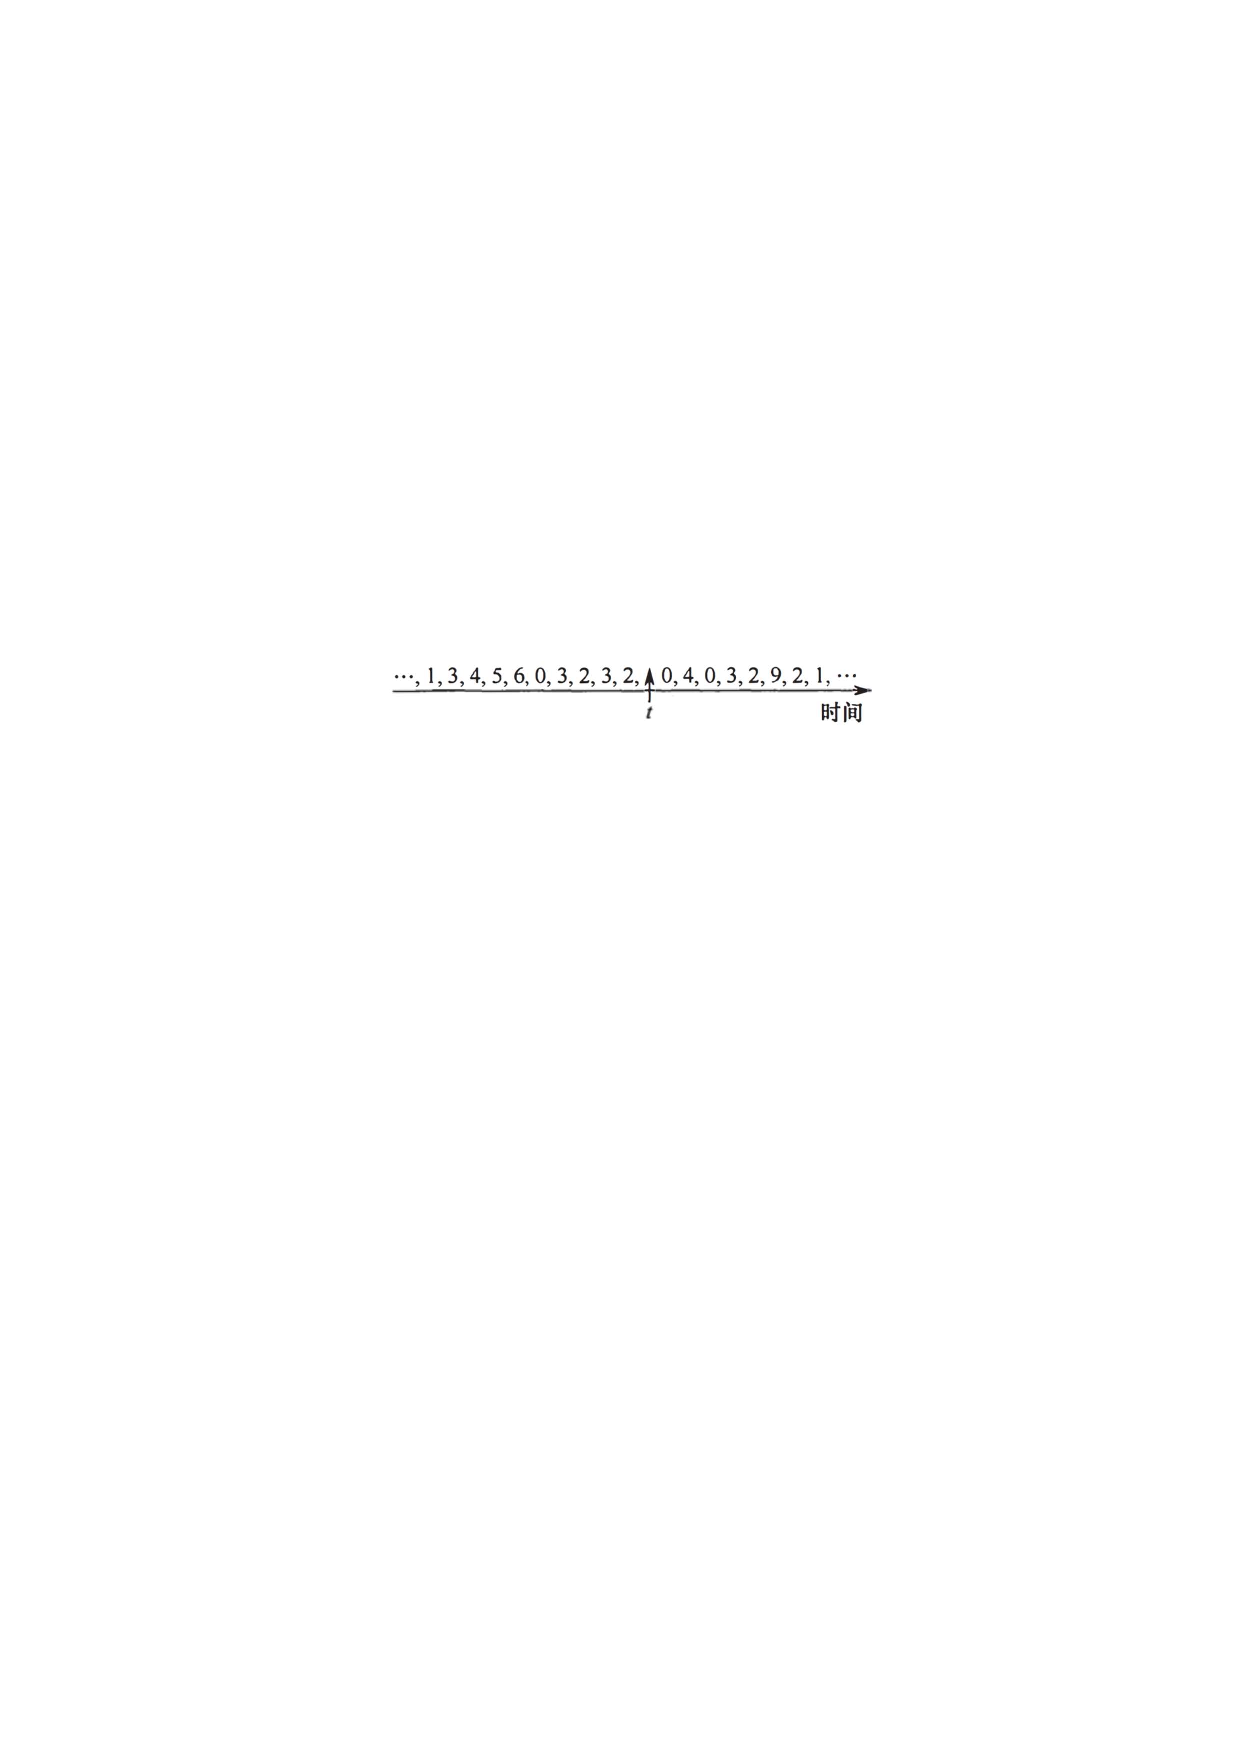
\includegraphics[width=.65\linewidth,height=.4\textheight,keepaspectratio]{../assets/figures/2016-questions-p004-b006.pdf}\end{center}

30. 进程 \(\displaystyle P_1\) 和 \(\displaystyle P_2\) 均包含并发执行的线程，部分伪代码描述如下所示。


\begin{Verbatim}[breaklines,breakanywhere,fontsize=\small]
// 进程 P1
int x = 0;
Thread1() { int a; a=1; x += 1; }
Thread2() { int a; a=2; x += 2; }
\end{Verbatim}

\begin{Verbatim}[breaklines,breakanywhere,fontsize=\small]
// 进程 P2
int x = 0;
Thread3() { int a; a=x; x += 3; }
Thread4() { int b
    b=x; x += 4; }
\end{Verbatim}

下列选项中，需要互斥执行的操作是\_\_\_\_\_\_。


\begin{center}\begin{tabular}{>{\raggedright\arraybackslash}p{\dimexpr(\linewidth-8\tabcolsep)/4\relax}>{\raggedright\arraybackslash}p{\dimexpr(\linewidth-8\tabcolsep)/4\relax}>{\raggedright\arraybackslash}p{\dimexpr(\linewidth-8\tabcolsep)/4\relax}>{\raggedright\arraybackslash}p{\dimexpr(\linewidth-8\tabcolsep)/4\relax}}
\textbf{A.} a=1 与 a=2 & \textbf{B.} a=x 与 b=x & \textbf{C.} x+=1 与 x+=2 & \textbf{D.} x+=1 与 x+=3\\[.35em]\end{tabular}\end{center}

31.下列关于SPOOLing 技术的叙述中，错误的是\_\_\_\_\_\_。


\begin{center}\begin{tabular}{>{\raggedright\arraybackslash}p{\dimexpr(\linewidth-4\tabcolsep)/2\relax}>{\raggedright\arraybackslash}p{\dimexpr(\linewidth-4\tabcolsep)/2\relax}}
\textbf{A.} 需要外存的支持 & \textbf{B.} 需要多道程序设计技术的支持\\[.35em]
\textbf{C.} 可以让多个作业共享一台独占设备 & \textbf{D.} 由用户作业控制设备与输入/输出井之间的数据传送\\[.35em]\end{tabular}\end{center}

32.下列关于管程的叙述中，错误的是\_\_\_\_\_\_。


\begin{center}\begin{tabular}{>{\raggedright\arraybackslash}p{\dimexpr(\linewidth-4\tabcolsep)/2\relax}>{\raggedright\arraybackslash}p{\dimexpr(\linewidth-4\tabcolsep)/2\relax}}
\textbf{A.} 管程只能用于实现进程的互斥 & \textbf{B.} 管程是由编程语言支持的进程同步机制\\[.35em]
\textbf{C.} 任何时候只能有一个进程在管程中执行 & \textbf{D.} 管程中定义的变量只能被管程内的过程访问 题33～41 均依据题33～41 图回答。\\[.35em]\end{tabular}\end{center}

33.在OSI 参考模型中，RI、Switch、Hub 实现的最高功能层分别是\_\_\_\_\_\_。


\begin{center}\begin{tabular}{>{\raggedright\arraybackslash}p{\dimexpr(\linewidth-8\tabcolsep)/4\relax}>{\raggedright\arraybackslash}p{\dimexpr(\linewidth-8\tabcolsep)/4\relax}>{\raggedright\arraybackslash}p{\dimexpr(\linewidth-8\tabcolsep)/4\relax}>{\raggedright\arraybackslash}p{\dimexpr(\linewidth-8\tabcolsep)/4\relax}}
\textbf{A.} 2、2、1 & \textbf{B.} 2、2、2 & \textbf{C.} 3、2、1 & \textbf{D.} 3、2、2\\[.35em]\end{tabular}\end{center}

34. 若连接和 R3 链路的频率带宽为 8kHz，信噪比为 30dB，该链路实际数据传输速率约为理论最大数据传输速率的 50\%。则该链路的实际数据传输速率约是\_\_\_\_\_\_。


\begin{center}\begin{tabular}{>{\raggedright\arraybackslash}p{\dimexpr(\linewidth-8\tabcolsep)/4\relax}>{\raggedright\arraybackslash}p{\dimexpr(\linewidth-8\tabcolsep)/4\relax}>{\raggedright\arraybackslash}p{\dimexpr(\linewidth-8\tabcolsep)/4\relax}>{\raggedright\arraybackslash}p{\dimexpr(\linewidth-8\tabcolsep)/4\relax}}
\textbf{A.} 8kbps & \textbf{B.} 20Kbps & \textbf{C.} 40kbps & \textbf{D.} 80kbps\\[.35em]\end{tabular}\end{center}

\begin{center}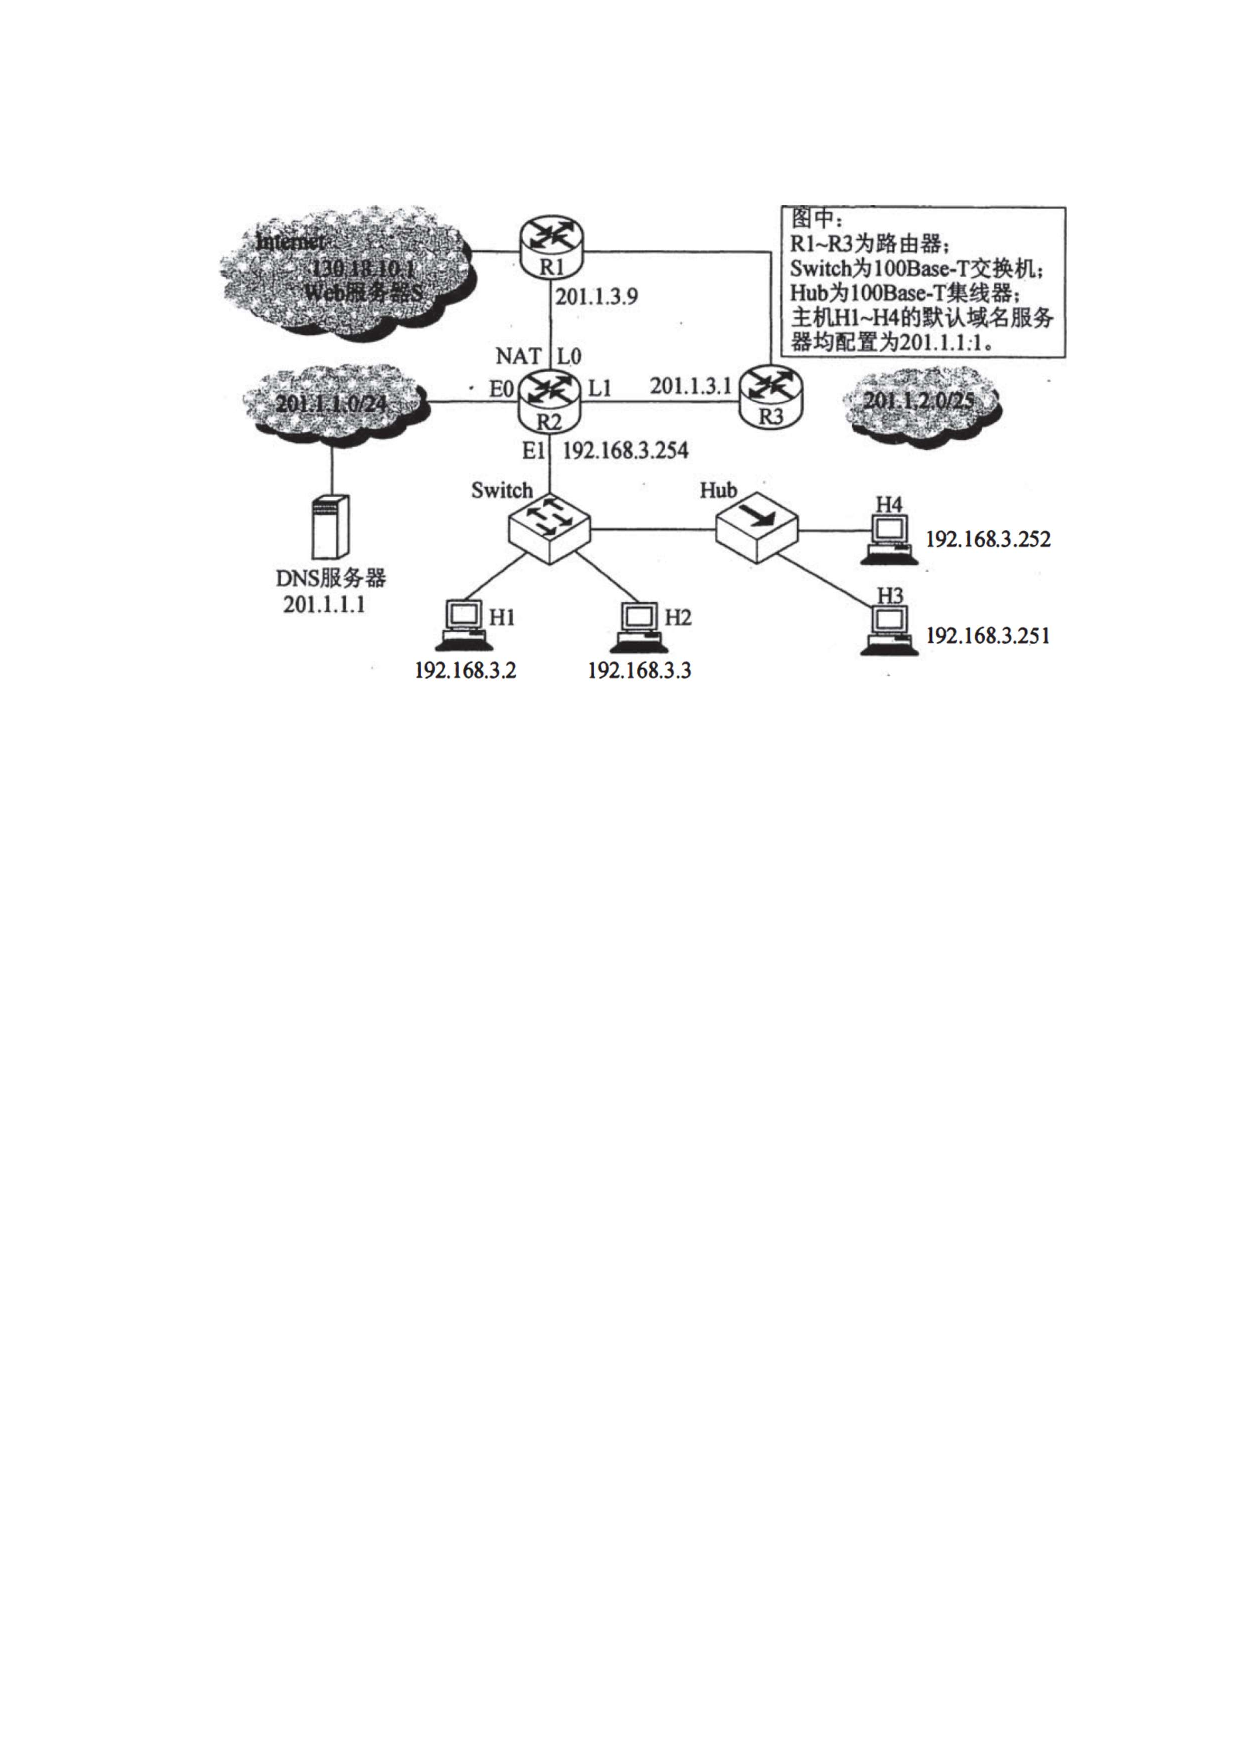
\includegraphics[width=.65\linewidth,height=.4\textheight,keepaspectratio]{../assets/figures/2016-questions-p005-b001.pdf}\end{center}

35.若主机H2 向主机H4 发送1 个数据帧，主机H4 向主机H2 立即发送一个确认帧，则除H4 外， 从物理层上能够收到该确认帧的主机还有 。


\begin{center}\begin{tabular}{>{\raggedright\arraybackslash}p{\dimexpr(\linewidth-8\tabcolsep)/4\relax}>{\raggedright\arraybackslash}p{\dimexpr(\linewidth-8\tabcolsep)/4\relax}>{\raggedright\arraybackslash}p{\dimexpr(\linewidth-8\tabcolsep)/4\relax}>{\raggedright\arraybackslash}p{\dimexpr(\linewidth-8\tabcolsep)/4\relax}}
\textbf{A.} 仅H2 & \textbf{B.} 仅H3 & \textbf{C.} 仅H1、H2 & \textbf{D.} 仅H2、H3\\[.35em]\end{tabular}\end{center}

36. 若 Hub 再生比特流过程中，会产生 \(\displaystyle 1.535\mu\mathrm{s}\) 延时，信号传播速度为 \(\displaystyle 200\mathrm{m}/\mu\mathrm{s}\)，不考虑以太网帧的前导码，则 H3 与 H4 之间理论上可以相距的最远距离是\_\_\_\_\_\_。


\begin{center}\begin{tabular}{>{\raggedright\arraybackslash}p{\dimexpr(\linewidth-8\tabcolsep)/4\relax}>{\raggedright\arraybackslash}p{\dimexpr(\linewidth-8\tabcolsep)/4\relax}>{\raggedright\arraybackslash}p{\dimexpr(\linewidth-8\tabcolsep)/4\relax}>{\raggedright\arraybackslash}p{\dimexpr(\linewidth-8\tabcolsep)/4\relax}}
\textbf{A.} 200m & \textbf{B.} 205m & \textbf{C.} 359m & \textbf{D.} 512m\\[.35em]\end{tabular}\end{center}

37. 假设 R1、R2、R3 采用 RIP 协议交换路由信息，且均已收敛。若 R3 检测到网络 201.1.2.0/25 不可达，并向通告一次新的距离向量，则 R2 更新后，其到达该网络的距离是\_\_\_\_\_\_。


\begin{center}\begin{tabular}{>{\raggedright\arraybackslash}p{\dimexpr(\linewidth-8\tabcolsep)/4\relax}>{\raggedright\arraybackslash}p{\dimexpr(\linewidth-8\tabcolsep)/4\relax}>{\raggedright\arraybackslash}p{\dimexpr(\linewidth-8\tabcolsep)/4\relax}>{\raggedright\arraybackslash}p{\dimexpr(\linewidth-8\tabcolsep)/4\relax}}
\textbf{A.} 2 & \textbf{B.} 3 & \textbf{C.} 16 & \textbf{D.} 17\\[.35em]\end{tabular}\end{center}

38.假设连接R1、R2 和R3 之间的点对点链路使用201.1.3.x/30 地址，当H3 访问Web 服务器S 时，R2 转发出去的封装HTTP 请求报文的IP 分组的源IP 地址和目的IP 地址分别是\_\_\_\_\_\_。


\begin{center}\begin{tabular}{>{\raggedright\arraybackslash}p{\dimexpr(\linewidth-4\tabcolsep)/2\relax}>{\raggedright\arraybackslash}p{\dimexpr(\linewidth-4\tabcolsep)/2\relax}}
\textbf{A.} 192.\allowbreak{}168.\allowbreak{}3.\allowbreak{}251, 130.\allowbreak{}18.\allowbreak{}10.\allowbreak{}1 & \textbf{B.} 192.\allowbreak{}168.\allowbreak{}3.\allowbreak{}251, 201.\allowbreak{}1.\allowbreak{}3.\allowbreak{}9\\[.35em]
\textbf{C.} 201.\allowbreak{}1.\allowbreak{}3.\allowbreak{}8, 130.\allowbreak{}18.\allowbreak{}10.\allowbreak{}1 & \textbf{D.} 201.\allowbreak{}1.\allowbreak{}3.\allowbreak{}10, 130.\allowbreak{}18.\allowbreak{}10.\allowbreak{}1\\[.35em]\end{tabular}\end{center}

39.若H1 与H2 的默认网关和子网掩码均分别配置为192.168.3.1 和255.255.255.128，H3 和H4 的默 认网关和子网掩码均分别配置为192.168.3.254 和255.255.255.128，则下列现象中可能发生的 是\_\_\_\_\_\_。


\begin{center}\begin{tabular}{>{\raggedright\arraybackslash}p{\dimexpr(\linewidth-4\tabcolsep)/2\relax}>{\raggedright\arraybackslash}p{\dimexpr(\linewidth-4\tabcolsep)/2\relax}}
\textbf{A.} H1 不能与H2 进行正常IP 通信 & \textbf{B.} H2 与H4 均不能访问Internet\\[.35em]
\textbf{C.} H1 不能与H3 进行正常IP 通信 & \textbf{D.} H3 不能与H4 进行正常IP 通信\\[.35em]\end{tabular}\end{center}

40.假设所有域名服务器均采用迭代查询方式进行域名解析。当H4 访问规范域名为 www.abc.xyz.com 的网站时，域名服务器201.1.1.1 完成该域名解析过程中，可能发出DNS 查询 的最少和最多次数分别是\_\_\_\_\_\_。


\begin{center}\begin{tabular}{>{\raggedright\arraybackslash}p{\dimexpr(\linewidth-8\tabcolsep)/4\relax}>{\raggedright\arraybackslash}p{\dimexpr(\linewidth-8\tabcolsep)/4\relax}>{\raggedright\arraybackslash}p{\dimexpr(\linewidth-8\tabcolsep)/4\relax}>{\raggedright\arraybackslash}p{\dimexpr(\linewidth-8\tabcolsep)/4\relax}}
\textbf{A.} 0，3 & \textbf{B.} 1，3 & \textbf{C.} 0，4 & \textbf{D.} 1，4\\[.35em]\end{tabular}\end{center}

\subsection*{二、综合应用题（第 41～47 小题，共 70 分）}

41.（9 分）假设题33～41 图中的H3 访问Web 服务器S 时，S 为新建的TCP 连接分配了20KB（K = 1024）的接收缓存，最大段长MSS=1KB，平均往返时间RTT = 200ms。H3 建立连接时的初始 序号为100，且持续以MSS 大小的段向S 发送数据，拥塞窗口初始阈值为32KB；S 对收到的每 个段进行确认，并通告新的接收窗口。假定TCP 连接建立完成后，S 端的TCP 接收缓存仅有数 据存入而无数据取出。请回答下列问题。 （1）在TCP 连接建立过程中，H3 收到的S 发送过来的第二次握手TCP 段的SYN 和ACK 标志 位的值分别是多少？确认序号是多少？ （2）H3 收到的第8 个确认段所通告的接收窗口是多少？此时H3 的拥塞窗口变为多少？H3 的 发送窗口变为多少？ （3）当H3 的发送窗口等于0 时，下一个待发送的数据段序号是多少？H3 从发送第1 个数据段 到发送窗口等于0 时刻为止，平均数据传输速率是多少（忽略段的传输延时）？ （4）若H3 与S 之间通信己经结束，在t 时刻H3 请求断开该连接，则从t 时刻起，S 释放该连 接的最短时间是多少？


42. （8 分）如果一棵非空 \(\displaystyle k\;(k\ge2)\) 叉树 T 中每个非叶结点都有 \(\displaystyle k\) 个孩子，则称 T 为正则 \(\displaystyle k\) 叉树。请回答下列问题并给出推导过程。（1）若 T 有 \(\displaystyle m\) 个非叶结点，则 T 中的叶结点有多少个？（2）若 T 的高度为 \(\displaystyle h\)（单结点的树 \(\displaystyle h=1\)），则 T 的结点数最多为多少个？最少为多少个？


43. （15 分）已知由 \(\displaystyle n\;(n\ge2)\) 个正整数构成的集合 \(\displaystyle A=\{a_k\mid0\le k<n\}\)，将其划分为两个不相交的子集 \(\displaystyle A_1\) 和 \(\displaystyle A_2\)，元素个数分别是 \(\displaystyle n_1\) 和 \(\displaystyle n_2\)，\(\displaystyle A_1\) 和 \(\displaystyle A_2\) 中元素之和分别为 \(\displaystyle S_1\) 和 \(\displaystyle S_2\)。设计一个尽可能高效的划分算法，满足 \(\displaystyle |n_1-n_2|\) 最小且 \(\displaystyle |S_1-S_2|\) 最大。要求：（1）给出算法的基本设计思想。（2）根据设计思想，采用 C 或 C++ 语言描述算法，关键之处给出注释。（3）说明你所设计算法的平均时间复杂度和空间复杂度。


44.（9 分）假定CPU 主频为50MHz，CPI 为4。设备D 采用异步串行通信方式向主机传送7 位 ASCII 字符，通信规程中有1 位奇校验位和1 位停止位，从D 接收启动命令到字符送入I/O 端口 需要0.5ms。请回答下列问题，要求说明理由。 （1）每传送一个字符，在异步串行通信线上共需传输多少位？在设备D 持续工作过程中，每秒 钟最多可向I/O 端口送入多少个字符？ （2）设备D 采用中断方式进行输入/输出，示意图如下。 I/O 端口每收到一个字符申请一次中断，中断响应需10 个时钟周期，中断服务程序共有20 条 指令，其中第15 条指令启动D 工作。若CPU 需从D 读取1000 个字符，则完成这一任务所需时 间大约是多少个时钟周期？CPU 用于完成这一任务的时间大约是多少个时钟周期？在中断响应阶 段CPU 进行了哪些操作？


\begin{center}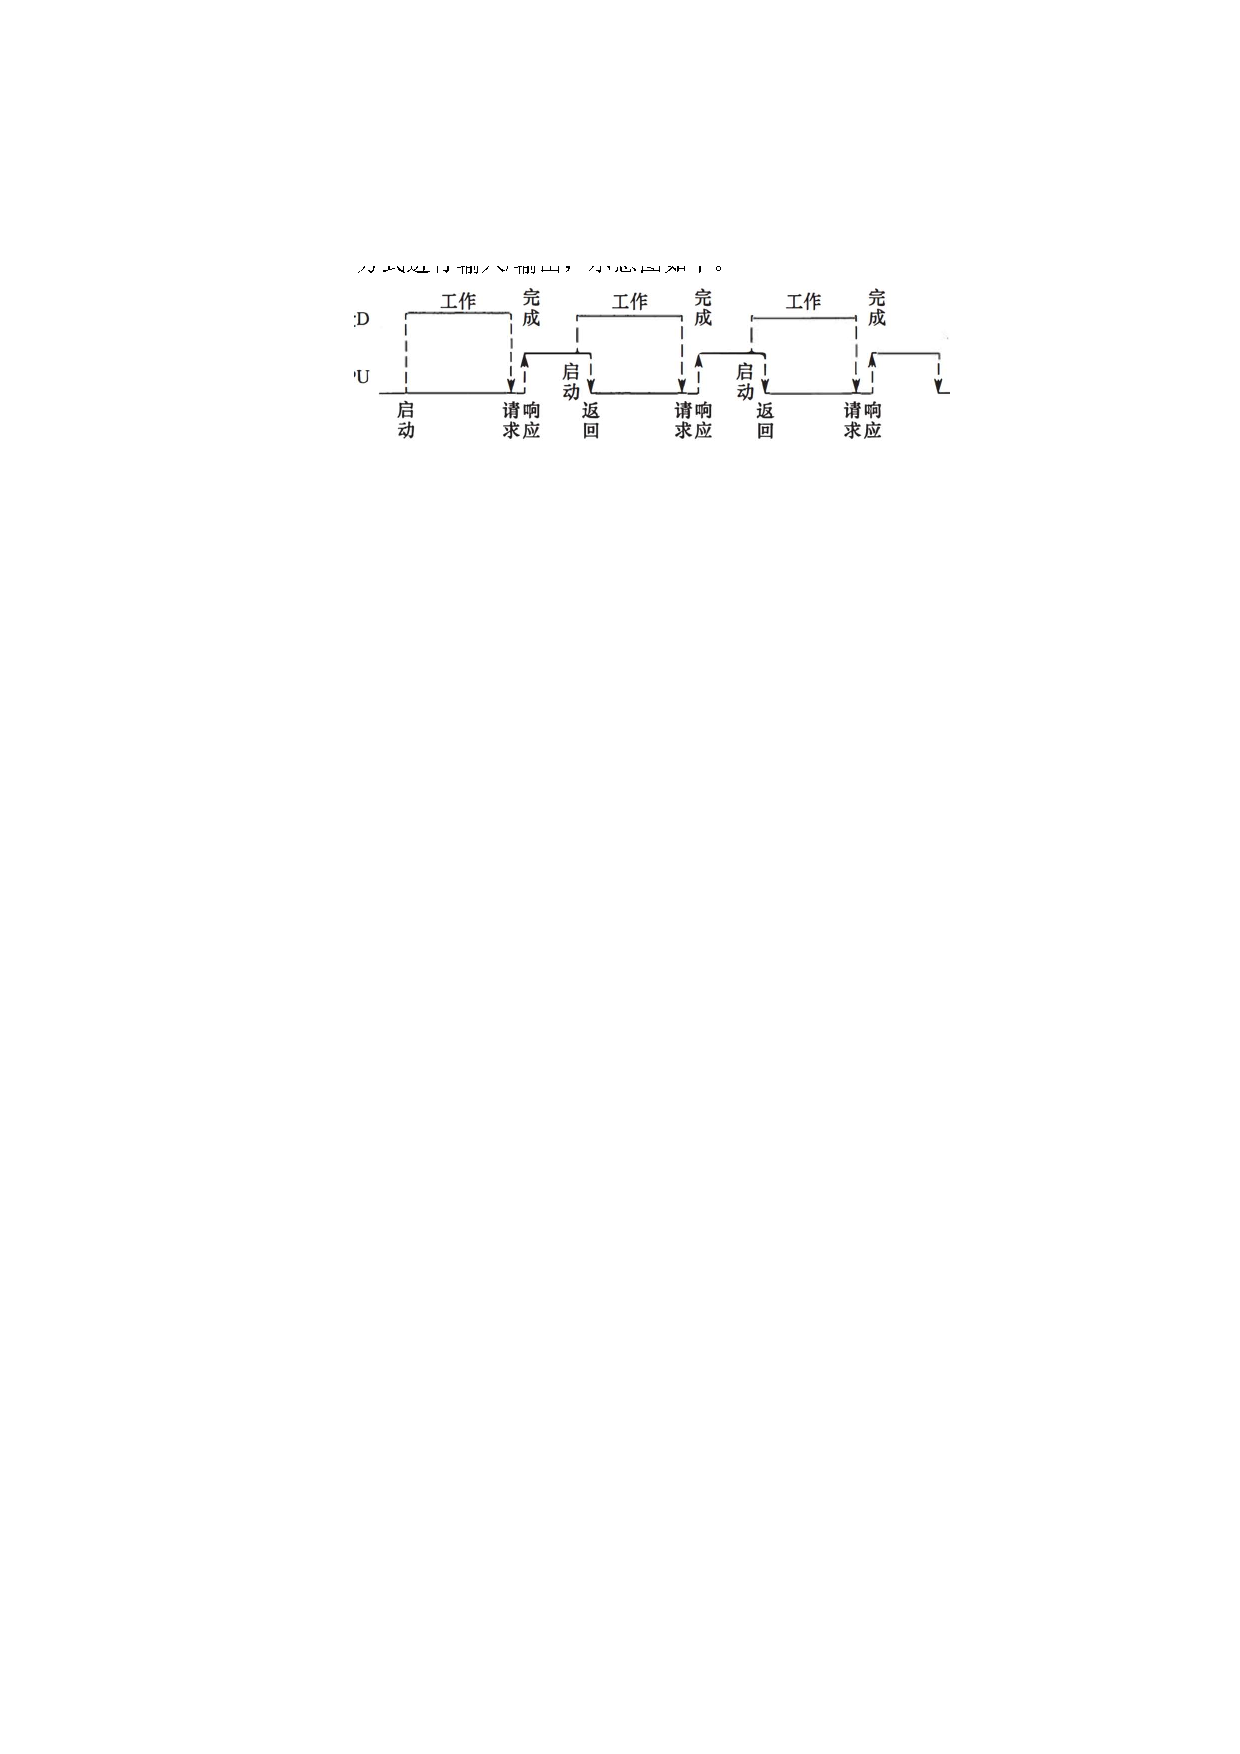
\includegraphics[width=.65\linewidth,height=.4\textheight,keepaspectratio]{../assets/figures/2016-questions-p009-b001.pdf}\end{center}

45.（14 分）某计算机采用页式虚拟存储管理方式，按字节编址，虚拟地址为32 位，物理地址为24 位，页大小为8KB；TLB 采用全相联映射：Cache 数据区大小为64KB，按2 路组相联方式组 织，主存块大小为64B。存储访问过程的示意图如下。 请回答下列问题。 （1）图中字段A～G 的位数各是多少？TLB 标记字段B 中存放的是什么信息？ （2）将块号为4099 的主存块装入到Cache 中时，所映射的Cache 组号是多少？对应的H 字段内容是什么？ （3）Cache 缺失处理的时间开销大还是缺页处理的时间开销大？为什么？ （4）为什么cache 可以采用直写（Write Through）策略，而修改页面内容时总是采用回写 （Write Back）策略。


\begin{center}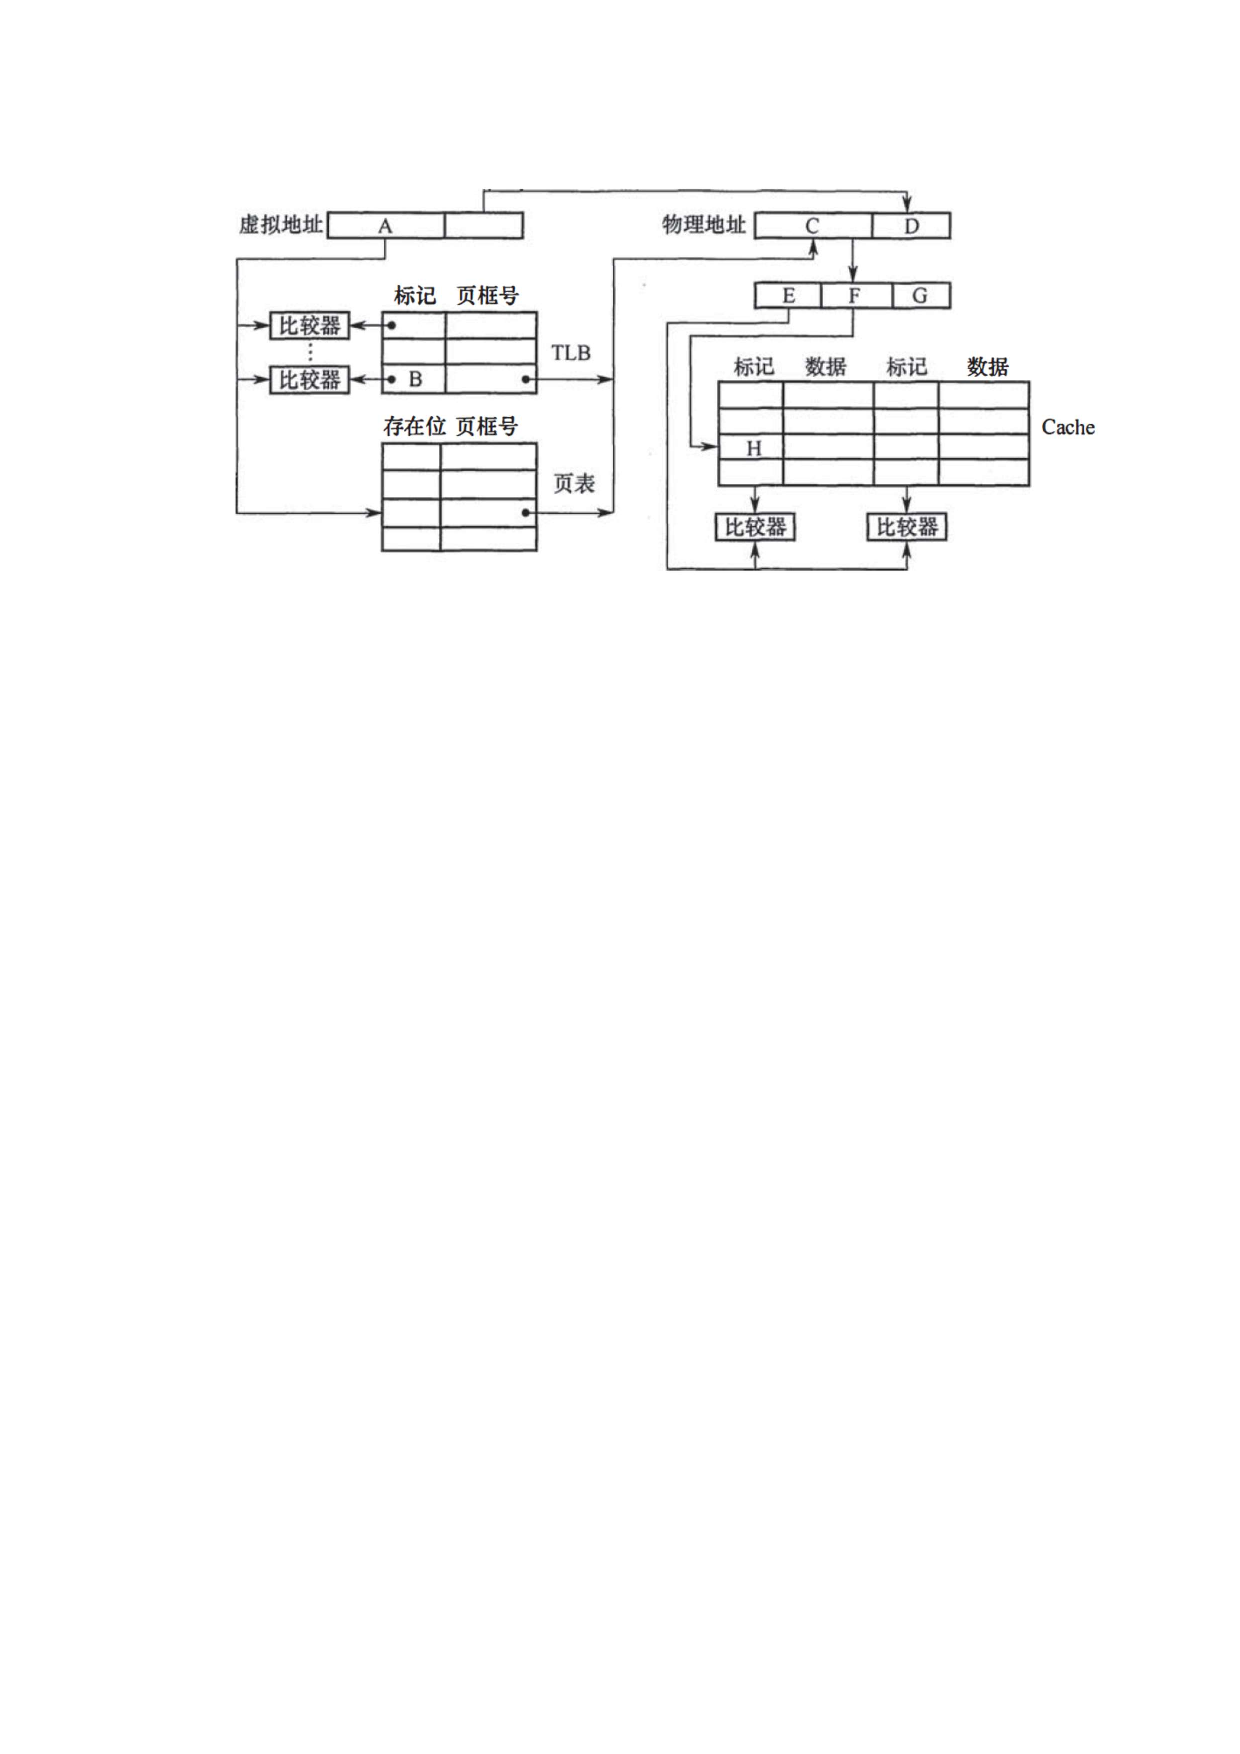
\includegraphics[width=.65\linewidth,height=.4\textheight,keepaspectratio]{../assets/figures/2016-questions-p010-b001.pdf}\end{center}

46.（6 分）某进程调度程序采用基于优先数（priority）的调度策略，即选择优先数最小的进程运 行，进程创建时由用户指定一个nice 作为静态优先数。为了动态调整优先数，引入运行时间 cpuTime 和等待时间waitTime，初值均为0。进程处于执行态时，cpuTime 定时加1，且 waitTime 置0；进程处于就绪态时，cpuTime 置0，waitTime 定时加1。请回答下列问题。 （1）若调度程序只将nice 的值作为进程的优先数，即priority = nice，则可能会出现饥饿现象， 为什么？ （2）使用nice、cpuTime 和waitTime 设计一种动态优先数计算方法，以避免产生饥饿现象，并 说明waitTime 的作用。


47. （9 分）磁盘文件系统使用链接分配方式组织文件，簇大小为 4KB。目录文件的每个目录项包括文件名和文件的第一个簇号，其他簇号存放在文件分配表 FAT 中。（1）假定目录树如下图所示，各文件占用的簇号及顺序如右表所示，其中 dir、dir1 是目录，file1、file2 是用户文件。请给出所有目录文件的内容。


\begin{center}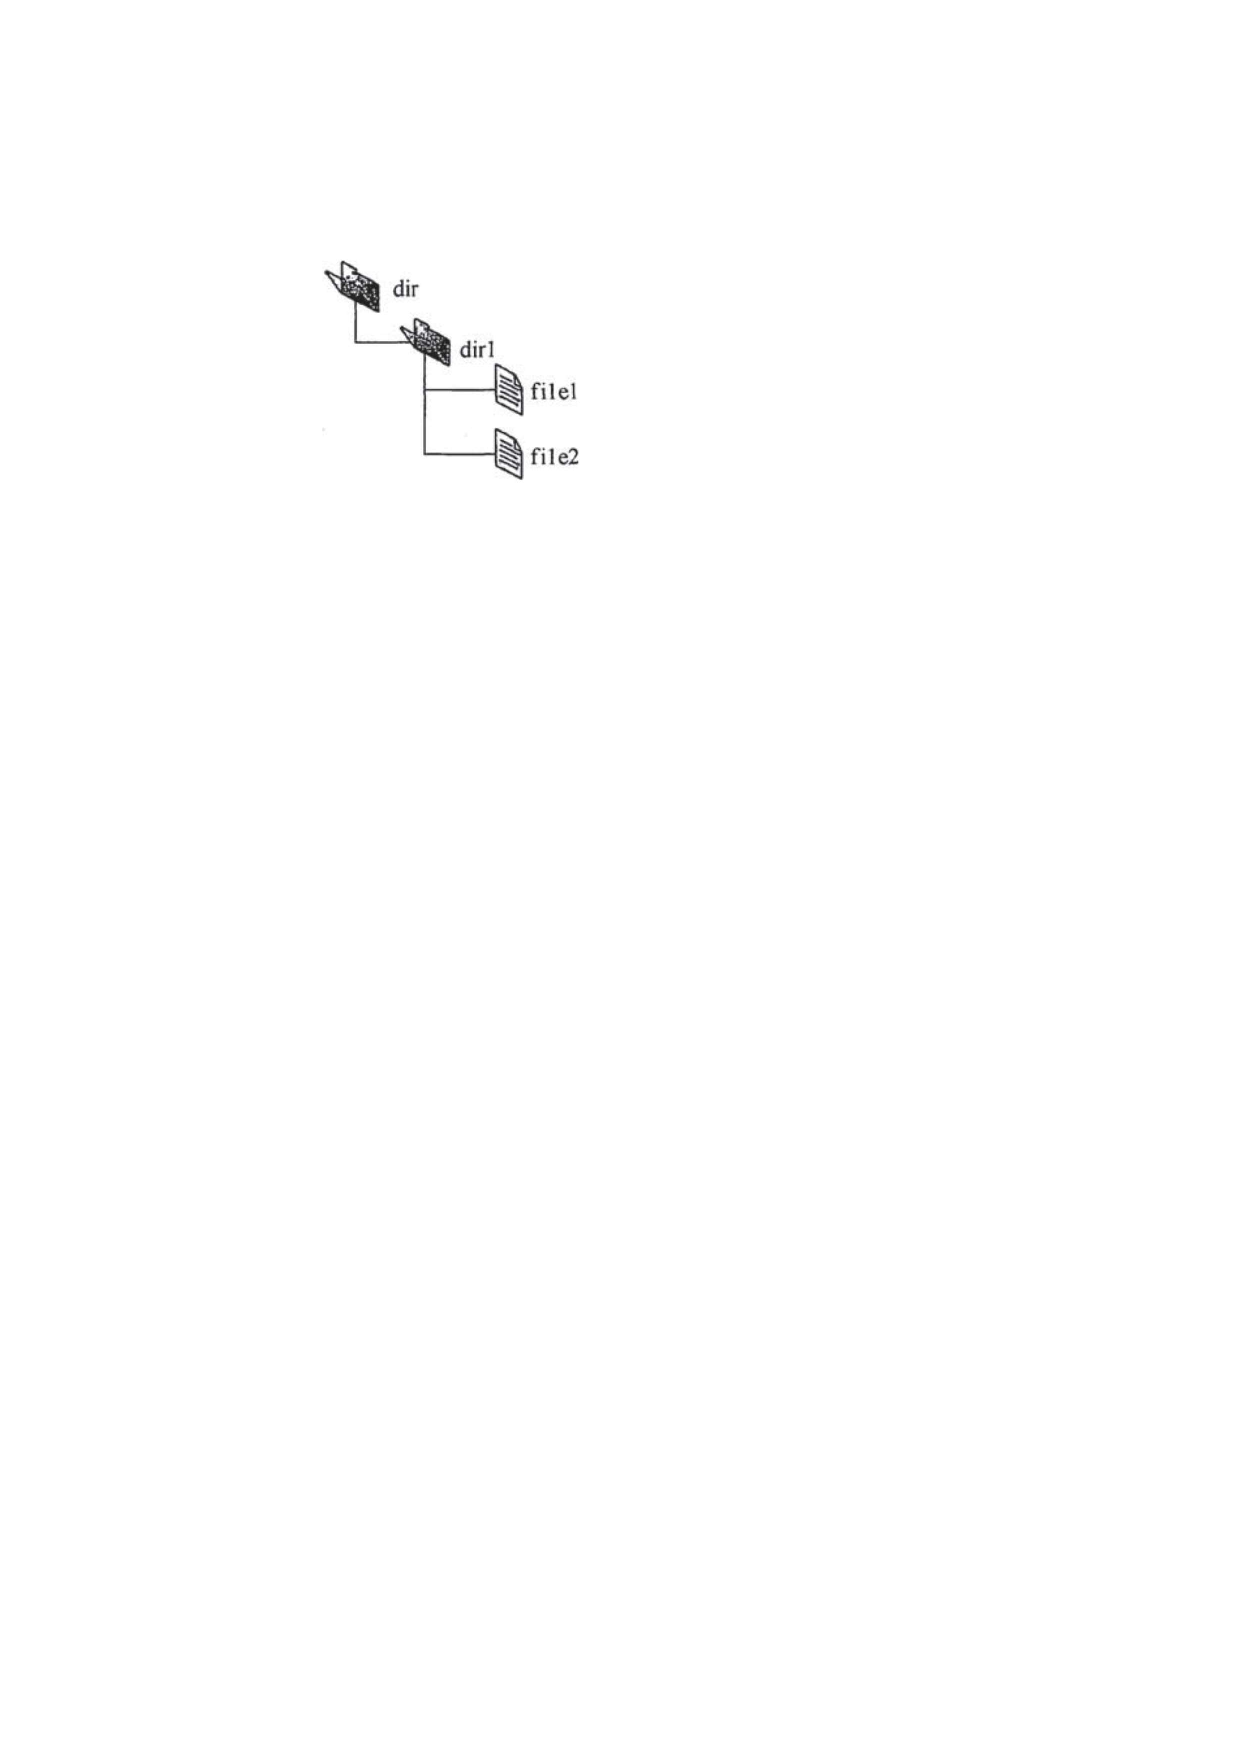
\includegraphics[width=.65\linewidth,height=.4\textheight,keepaspectratio]{../assets/figures/2016-questions-p012-b001.pdf}\end{center}

\begin{center}\begin{adjustbox}{max width=\linewidth}\begin{tabular}{|>{\raggedright\arraybackslash}p{\dimexpr(\linewidth-4\tabcolsep-3\arrayrulewidth)/2\relax}|>{\raggedright\arraybackslash}p{\dimexpr(\linewidth-4\tabcolsep-3\arrayrulewidth)/2\relax}|}\hline
文件名 & 簇号\\\hline
dir & 1\\\hline
dir1 & 48\\\hline
file1 & 100、106、108\\\hline
file2 & 200、201、202\\\hline\end{tabular}\end{adjustbox}\end{center}

（2）若 FAT 的每个表项仅存放簇号，占 2 字节，则 FAT 的最大长度为多少字节？该文件系统支持的文件长度最大是多少？（3）系统通过目录文件和 FAT 实现对文件的按名存取，说明 file1 的 106、108 两个簇号分别存放在 FAT 的哪个表项中。（4）假设仅 FAT 和 dir 目录文件已读入内存，若需将文件 dir/dir1/file 的第 50 个字节读入内存，则要访问哪几个簇？

\end{document}
